\chapter{模板的使用}
首先不要被一些可能陌生的名词吓倒。本模板的理念是以实用为目的,能让文科甚至完全零基础的同学也可以从繁复的格式设置中解放出来,专注于文章内容。因此,只要认真按照本文档学习,一定可以作出的完美的排版。当然,每个同学都有不同的毕业论文或设计,不可能面面俱到,如果遇到问题或有什么建议,请到我们的 project 里反映,地址是 \url{http://code.google.com/p/njubachelor/}。

\section{编译环境的准备}
要想使用本模板,首先需要在你的计算机上安装一个 \LaTeX{} 系统。关于其的一个简单介绍可以参考\href{http://zh.wikipedia.org/wiki/Latex}{维基百科}。鉴于目前在线编译不是特别成熟,所以我们仍然采用本地安装一套 \TeX{} 的排版系统。

根据你所采用的操作系统,请选择合适的发行版:
\begin{itemize}
	\item Mac OS: \url{http://www.tug.org/mactex/}
	\item Windows: \url{http://www.ctex.org/CTeXDownload},基于 MiKTeX;CTeX 套装使用方便。
	\item Linux: 使用 Linux 的同学应该没必要在这里浪费时间,你们直接做你们想要做的吧。
\end{itemize}
CTeX 发行版又分为基本版 Basic 和完整版 Full,你可以试试基本版可不可以顺利使用,并给我们反馈,初学者推荐安装完整版。顺利安装后系统会自动与 .tex 即 \LaTeX{} 源文件进行关联。双击便可以打开已安装好的 \TeX{} 文本编辑器,比如 OS X 下的 TeXWorks,CTeX 套装里的 WinEdt 进行修改和编译。请先打开本模板里的 test.tex,你可以简单熟悉一下 \LaTeX{} 的源文件结构,并试一下编译,看看生成的 test.pdf 效果是能和自带的 test-compare.pdf 是否一致(编译顺序为 XeLaTeX $\rightarrow$ BibTeX $\rightarrow$ XeLaTeX $\rightarrow$ XeLaTeX)。

\section{文件结构}
模板中文类 NJUbachelor.cls 是按南京大学本科毕业论文撰写和装订要求进行的格式设置文件,YourPaper.bst 是参考文献格式设置文件,YourPaper.tex 是你要编译的主文件,文件夹 frontmatter 下面的 abstract.tex 用来书写中英文摘要,文件夹 chapter 下 chapter1.tex, chapter2.tex \ldots 用来书写正文章节,文件夹 refs 下 refernces.bib 管理参考文献,figures 下保存所有要插入的图片,backmatter 下 acknowledgment.tex 和 appendices.tex 分别是致谢和附录,njulogos 下存放封面上使用的学校标志。.cls、.bst、.tex、.bib 格式的文件都可以用文本编辑器或合适的软件打开。

\section{基本要素}
虽然对 \LaTeX{} 完全不了解也不影响使用本模板,但是如果可以了解其基础知识,那么可以事半功倍。这里推荐入门必读里 lshort 这篇文档,若要更高级使用请参考“进一步阅读”部分。

论文的写作,有一些基本要素是经常使用的,比如论文标题、摘要、目录、分级标题、表格、注释、插图、列表、公式、参考文献、附录等。这里将这些基本元素的写法给出,你可以参考模板中各个 .tex 源文件的代码进行修改、试验、学习和使用。

\subsection{论文标题}
论文标题等一些个人信息涵盖在封面中,只需要打开 YourPaper.tex 将适当信息修改为你的即可。

\subsection{摘要}
将 abstract.tex 的相应信息替换即可。

\subsection{目录}
目录部分由编译时自动生成。

\subsection{分级标题}
用法如表 \ref{tab:fjbt} 所示。
{\zihao{5}
\begin{longtable}{cc}
	\caption{分级标题使用命令}\label{tab:fjbt}\\
	\midrule
	标题名称&	代码\\
	\hline
	大(章)标题&	\verb|\chapter{你的大(章)标题内容}|\\
	次级标题&	\verb|\chapter{你的次级标题内容}|\\
	三级标题&	\verb|\chapter{你的三级标题内容}|\\
	四级标题&	\verb|\chapter{你的四级标题内容}|\\
	\bottomrule
\end{longtable}
}

\subsection{表格}
其实,使用 \LaTeX{} 制作表格并不是特别方便,\LaTeX{} 最方便的地方在于数学公式的编排以及层次逻辑。这里我们仅以科技文献中最常用的“三线表”为例进行说明。比如上面的表 \ref{tab:fjbt},它的代码如下:
\begin{Verbatim}[frame=single]
{\zihao{5}
\begin{longtable}{cc}
	\caption{分级标题使用命令}\label{tab:fjbt}\\
	\midrule
	标题名称&	代码\\
	\hline
	大(章)标题&	\verb|\chapter{你的大(章)标题内容}|\\
	次级标题&	\verb|\chapter{你的次级标题内容}|\\
	三级标题&	\verb|\chapter{你的三级标题内容}|\\
	四级标题&	\verb|\chapter{你的四级标题内容}|\\
	\bottomrule
\end{longtable}
}
\end{Verbatim}
其中,\verb|{\zihao{5}…}| 是为了符合学校要求表格使用 5 号字,你如果不想理会学校可以不用使用此命令。然后

还有一种解决办法是用其他软件生成表格并保存成图片,以图片形式插入,关于图片插入请参考 \ref{text:picture}。更进一步学习表格请参考“进一步阅读”部分。

\subsection{注释}
注释采用脚注,使用起来很简单\footnote{就像这样。}。只需要在你要加注释的地方用即可。比如第一句的源代码为
\begin{Verbatim}[frame=single]
注释采用脚注,使用起来很简单\footnote{就像这样。}。
\end{Verbatim}
这全都是自动的(标号、生成),一切不用你多操心\footnote{真得很简单吧。}。

\subsection{插图}
插个图试试:
\begin{figure}[!h]
	\centering
	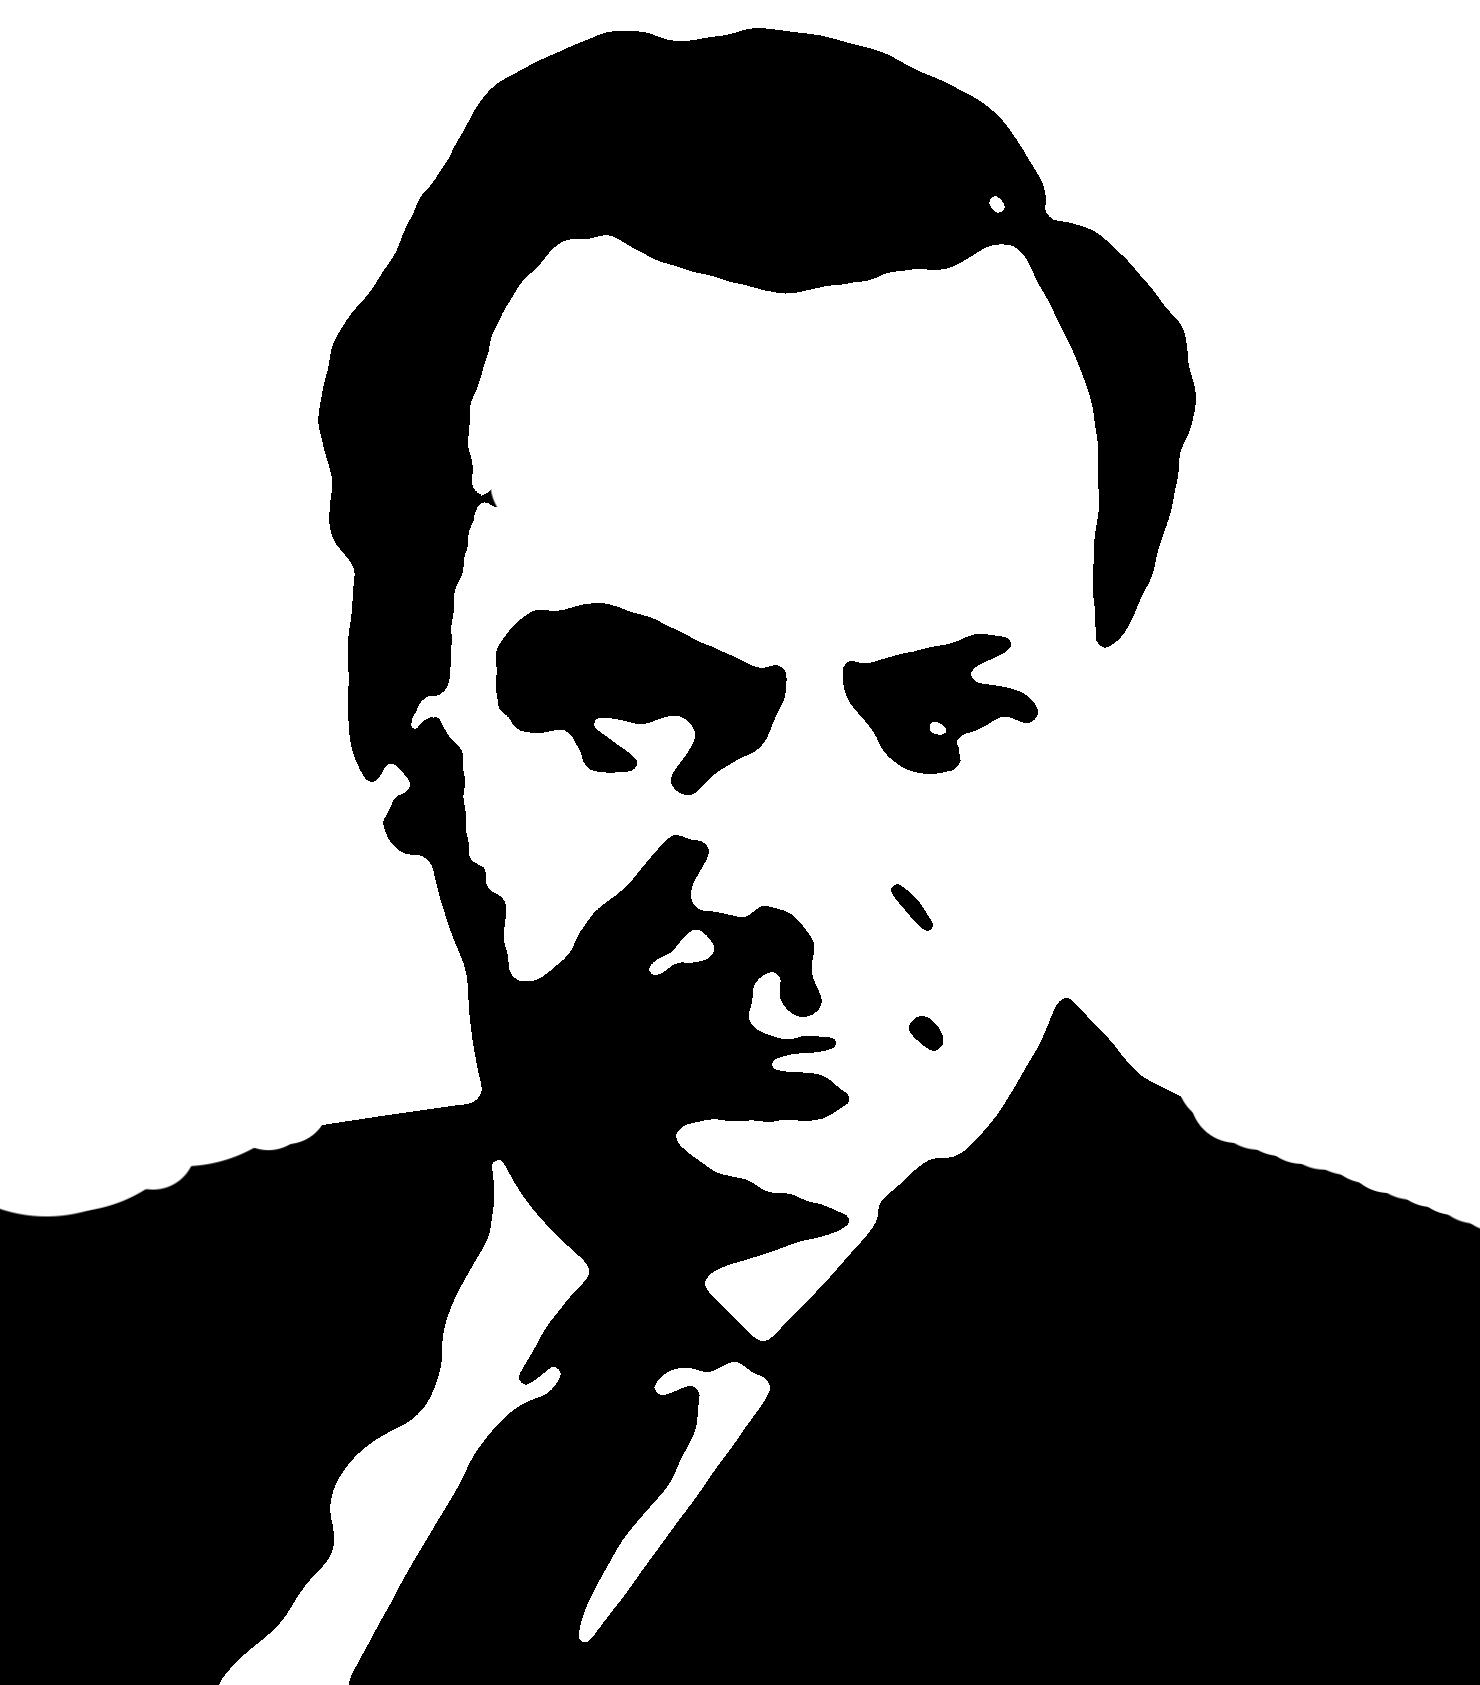
\includegraphics[height=4cm]{figures/feynman.png}
	\caption{这是一个测试: Dr. Feynman}\label{fig:feynman}
\end{figure}

\subsection{列表}
列表就是列举、枚举。

\subsection{公式}

\subsection{参考文献}

\subsection{附录}

